\documentclass[../../main]{subfiles}

\begin{document}
\chapter{測度空間}

\section{イントロダクション}

\cref{chapter:hilbert_space},\cref{chapter:probability_space}では,関数空間での直交射影を積分に基づいて論じた.
関数空間でも直交射影を定義できる理由は,\(\Lebesgue{2}(\Omega)=\Set{f\given\int_\Omega\abs{f(x)}^2\intd{x}<+\infty}\)がヒルベルト空間,つまり,完備な内積空間だからである.
そして,\(\Lebesgue{2}(\Omega)\)の完備性には,積分がリーマン積分ではなくルベーグ積分であることが効いている.

また,確率変数の期待値はルベーグ積分で定義される.これは,ルベーグ積分を使うと関数の定義域をより自由に選べることの恩恵である.まとめると,ルベーグ積分はリーマン積分に次の2点で優る.
\begin{enumerate}
  \item 積分と極限の相性がよい.
  \item 関数の定義域が\(\numset{R}^n\)の部分集合でなくともよい.
\end{enumerate}

これらの強みは主に,ルベーグ積分では面積の測り方(測度)を自由に決められること,そして,測度の観点から区別できないものは同一視できることに由来する.言い換えると,ルベーグ積分のメリットを存分に享受するには
\begin{enumerate}
  \item 面積が定義される集合のあつまり(\impact{σ‐加法族})を用意する.
  \item 各集合に面積を割り当てる写像(\impact{測度})を用意する.
  \item 積分を定義できる関数(\impact{可測関数})を規定する.
\end{enumerate}
という,3つの段階を要する.本章では,この3ステップをどう踏んでいけばよいのかを,かけ足で概観する.

\section{測度論の基本概念}

\subsection{σ‐加法族}

\begin{definition}{σ‐加法族}{sigma_algebra}\index{しぐまかほうぞく@σ‐加法族}
  \(\Omega\)を集合,\(\sigmaalg{F}\)を\(\powerset{\Omega}\)の部分集合とする.
  \(\sigmaalg{F}\)が\(\Omega\)上の\termdef{σ‐加法族}(σ‐algebra)であるとは,\(\sigmaalg{F}\)が以下の条件を満たすことをいう.
  \begin{enumerate}
    \item \(\Omega\in\sigmaalg{F}\)である.
    \item 任意の\(A\in\sigmaalg{F}\)に対して\(\scomp{A}=\Omega\setminus A\in\sigmaalg{F}\)である.
    \item 任意の\(A_1,A_2,\dotsc\in\sigmaalg{F}\)に対して\(\bigcup_{n\in\numset{N}}A_n\in\sigmaalg{F}\)である.
  \end{enumerate}
\end{definition}

組\((\Omega,\sigmaalg{F})\)を\termdef{可測空間}\index{かそくくうかん@可測空間}(measurable space)という.

\begin{example}
  \(\Set{\emptyset,\Omega}\)と\(\powerset{\Omega}\)は\(\Omega\)上のσ‐加法族である.
\end{example}

\begin{example}\label{example:dice}
  \(\Omega=\Set{\dicei,\diceii,\diceiii,\diceiv,\dicev,\dicevi}\)を6元集合とし,\(O=\Set{\dicei,\diceiii,\dicev}\)とおく.
  このとき,\(\sigmaalg{G}=\Set{\emptyset,O,\scomp{O},\Omega}\)は\(\Omega\)上のσ‐加法族である.
\end{example}

\begin{definition}{生成するσ‐加法族}{}\index{せいせい@生成!しぐまかほうぞく@σ‐加法族}\index{しぐまかほうぞく@σ‐加法族!せいせいする@生成する\twoemdash}\indexsymbol{\(\sigmagen{S}\)}
  \(\Omega\)を集合,\(S\)を\(\powerset{\Omega}\)の部分集合とする.また,\(S\)を包含する\(\Omega\)上のσ‐加法族全体を\(\Sigma(S)\)とおく.このとき,集合
  \[
    \sigmagen{S} = \bigcap_{\sigmaalg{F}\in\Sigma(S)}\sigmaalg{F}
  \]
  は\(\Sigma(S)\)に属し,\(\Sigma(S)\)の任意の元は\(\sigmagen{S}\)を包含する.\(\sigmagen{S}\)を\(S\)が\termdef{生成するσ‐加法族}(generated σ‐algebra)という.
\end{definition}

\begin{example}[ボレル集合族]\index{ぼれるしゅうごうぞく@ボレル集合族}\index{BR@\(\borelset{\numset{R}}\)}
  左半開区間の全体集合\(S=\Set{\ocival{-\infty}{a}\given a\in\numset{R}}\)により生成されるσ‐加法族を\termdef{ボレル集合族}(Borel algebra)といい,\(\borelset{\numset{R}}\)と表記する.
\end{example}

\begin{note}
  \(\borelset{\numset{R}}\)は\(\numset{R}\)の開集合系が生成するσ‐加法族でもある.実はより一般に,位相空間の開集合系が生成するσ‐加法族のことをボレル集合族という.
\end{note}

\begin{example}
  \cref{example:dice}のσ‐加法族\(\sigmaalg{G}\)は\(\sigmaalg{G}=\sigmagen{\Set{O}}\)と書ける.
  実際,\(\sigmaalg{F}\)が\(\Set{O}\)を包含するσ‐加法族なら\(\scomp{O}\in\sigmaalg{F}\),\(\sigmaalg{G}\subset\sigmaalg{F}\)である.
  つまり,\(\sigmaalg{G}\)は\(\Set{O}\)を包含する最小のσ‐加法族だから,\(\sigmaalg{G}=\sigmagen{\Set{O}}\)である.
\end{example}

\subsection{ボレル測度とルベーグ測度}

\begin{definition}{拡大実数}{extended_real}\index{かくだいじっすう@拡大実数}\index{R@\(\extendedreal\)}
  \(\numset{R}\)に正負の無限大\(+\infty,-\infty\notin\numset{R}\)を加えた集合\(\extendedreal=\numset{R}\cup\Set{\pm\infty}\)を\termdef{拡大実数}(extended real number)という.
  各\(a\in\numset{R}\),\(x\in\extendedreal\)に対し,\(\pm\infty\)との演算を以下の通り定義する(複合同順).
  \begin{gather*}
    a+(\pm\infty) = (\pm\infty)+a = \pm\infty,
    \quad a-(\pm\infty) = \mp\infty, \\
    (\pm\infty)+(\pm\infty) = \pm\infty,
    \quad(\pm\infty)-(\mp\infty) = \pm\infty, \\
    \frac{a}{\pm\infty} = 0,
    \quad x\cdot(\pm\infty) = (\pm\infty)\cdot x = \begin{cases}\pm\infty & (x>0),\\ 0 & (x=0), \\ \mp\infty & (x<0)\end{cases}
  \end{gather*}
\end{definition}

\begin{note}
  \((\pm\infty)+(\mp\infty)\)や\((\pm\infty)-(\pm\infty)\)などは定義されない.要するに,\(\extendedreal\)上では不定形でない極限のみ計算できる.また,普通\(0\cdot(\pm\infty)\)は不定形だが,ここでは\(0\cdot(\pm\infty)=0\)と定義した.
\end{note}

\(\seq{A_n}_{n\in\numset{N}}\)を集合列とする.\(\seq{A_n}_{n\in\numset{N}}\)が\termdef{互いに素}\index{たがいにそ@互いに素}(disjoint)であるとは,
異なる任意の2数\(i,j\in\numset{N}\)に対して\(A_i\cap A_j=\emptyset\)であることをいう.
互いに素な集合の和であることを強調したいときは,和集合\(\bigcup_nA_n\)を\(\bigsqcup_nA_n\)とも書く\indexsymbol{\(A\sqcup B\)}.

\begin{definition}{測度}{measure}\index{そくど@測度}\index{そくど@測度}
  \(\sigmaalg{F}\)をσ‐加法族とする.写像\(\mu\colon\sigmaalg{F}\to\ccival{0}{+\infty}\)が\(\sigmaalg{F}\)上の\termdef{測度}(measure)であるとは,
  \(\mu\)が以下の条件を満たすことをいう.
  \begin{enumerate}
    \item \(\mu(\emptyset)=0\)である.
    \item \(\sigmaalg{F}\)上の集合列\(\seq{A_n}_{n\in\numset{N}}\)が互いに素であるとき,\(\mu(\bigsqcup_{n\in\numset{N}}A_n)=\sum_{n=1}^\infty\mu(A_n)\)である.
  \end{enumerate}
\end{definition}

3つ組\((\Omega,\sigmaalg{F},\mu)\)を\termdef{測度空間}\index{そくどくうかん@測度空間}(measure space)という.
特に\(\mu(\Omega)=1\)であるとき,\(\mu\)を\termdef{確率測度}\index{かくりつそくど@確率測度}\index{そくど@測度!かくりつ@確率\twoemdash}(probability measure),\((\Omega,\sigmaalg{F},\mu)\)を\termdef{確率空間}\index{かくりつくうかん@確率空間}(probability space)という.
また,確率空間のσ‐加法族\(\sigmaalg{F}\)に属する各元は\termdef{事象}\index{じしょう@事象}(event)と呼ばれる.

\begin{example}[計数測度]\index{けいすうそくど@計数測度}
  \(\sigmaalg{F}\)をσ‐加法族とする.また,各\(A\in\sigmaalg{F}\)に対して,\(A\)が有限集合のとき\(\mu(A)=\sizeof{A}\),無限集合のとき\(\mu(A)=+\infty\)とする.
  このとき\(\mu\)は\(\sigmaalg{F}\)上の測度になる.\(\mu\)を\termdef{計数測度}(counting measure)という.
\end{example}

\begin{example}[ディラック測度]\index{でぃらっくそくど@ディラック測度}
  \((\Omega,\sigmaalg{F})\)を可測空間とし,任意に\(x\in\Omega\)をとる.また,各\(A\in\sigmaalg{F}\)に対して,\(x\in A\)のとき\(\delta_x(A)=1\),\(x\notin A\)のとき\(\delta_x(A)=0\)とする.
  このとき\(\delta_x\)は\(\sigmaalg{F}\)上の測度になる.\(\delta_x\)を\termdef{ディラック測度}(Dirac measure)という.
\end{example}

\begin{example}\label{example:equally_possible}
  \(\Omega\)を\cref{example:dice}と同じにし,\(\sigmaalg{F}=\powerset{\Omega}\)とする.このとき,写像\(\prob\colon\sigmaalg{F}\to\ccival{0}{1}\),\(\prob(A)=(1/6)\sizeof{A}\)は\(\sigmaalg{F}\)上の確率測度である.
  \(\prob\)は「どの目が出るのも同様に確からしい(公平な)6面ダイスに関する確率」を表すと解釈できる.たとえば,奇数の目が出る確率は\(\prob(O)=1/2\)である.
\end{example}

\begin{definition}{有限加法族}{finite_additive_class}\index{ゆうげんかほうぞく@有限加法族}
  \(\Omega\)を集合,\(\sigmaalg{A}\)を\(\powerset{\Omega}\)の部分集合とする.
  \(\sigmaalg{A}\)が\(\Omega\)上の\termdef{有限加法族}(finitely additive class)であるとは,\(\sigmaalg{A}\)が以下の条件を満たすことをいう.
  \begin{enumerate}
    \item \(\Omega\in\sigmaalg{A}\)である.
    \item 任意の\(A\in\sigmaalg{A}\)に対して\(\scomp{A}=\Omega\setminus A\in\sigmaalg{A}\)である.
    \item 任意の\(A,B\in\sigmaalg{A}\)に対して\(A\cup B\in\sigmaalg{A}\)である.
  \end{enumerate}
\end{definition}

\begin{definition}{有限加法的測度}{finitely_additive_measure}\index{ゆうげんかほうてきそくど@有限加法的測度}\index{そくど@測度!ゆうげんかほうてき@有限加法的\twoemdash}
  \(\sigmaalg{A}\)を有限加法族とする.写像\(m\colon\sigmaalg{A}\to\ccival{0}{+\infty}\)が\(\sigmaalg{A}\)上の\termdef{有限加法的測度}(finitely additive measure)であるとは,
  \(m\)が以下の条件を満たすことをいう.
  \begin{enumerate}
    \item \(m(\emptyset)=0\)である.
    \item \(A,B\in\sigmaalg{A}\)が\(A\cap B=\emptyset\)を満たすとき,\(m(A\sqcup B)=m(A)+m(B)\)である.
  \end{enumerate}
\end{definition}

\begin{note}
  infiniteは「インフィニット」と読むが,finiteは「ファイナイト」と読む.
\end{note}

\begin{theorem}{ホップの拡張定理}{hopf_extension}\index{ほっぷのかくちょうていり@ホップの拡張定理}
  \(\sigmaalg{A}\)を集合\(\Omega\)上の有限加法族,\(m\)を\(\sigmaalg{A}\)上の有限加法的測度とする.このとき,以下の命題は同値である.
  \begin{enumerate}
    \item \(\sigmaalg{A}\)上の集合列\(\seq{A_n}_{n\in\numset{N}}\)が互いに素で\(A=\bigsqcup_{n\in\numset{N}}A_n\in\sigmaalg{A}\)を満たすとき,\(m(A)=\sum_{n=1}^\infty m(A_n)\)である.
    \item \(\sigmagen{\sigmaalg{A}}\)上の測度\(\mu\)で,任意の\(A\in\sigmaalg{A}\)に対して\(\mu(A)=m(A)\)を満たすものが存在する.
  \end{enumerate}
  さらに,\(\sigmaalg{A}\)上の集合列\(\seq{A_n}_{n\in\numset{N}}\)で\(m(A_n)<+\infty\),\(\bigcup_{n\in\numset{N}}A_n=\Omega\)を満たすものが存在するとき,\(\mu\)は一意である.
  これを\termdef{ホップの拡張定理}(Hopf extension theorem)という.
\end{theorem}

\begin{note}
  \(\sigmaalg{A}\)上の集合列\(\seq{A_n}_{n\in\numset{N}}\)で\(m(A_n)<+\infty\),\(\bigcup_{n\in\numset{N}}A_n=\Omega\)を満たすものが存在するとき,
  \(m\)は\termdef{σ‐有限}\index{しぐまゆうげん@σ‐有限}(σ‐finite)であるという.本書が扱う(有限加法的)測度はすべてσ‐有限なので,\cref{theorem:hopf_extension}から定まる拡張された測度は常に一意である.
\end{note}

\begin{proof}
証明のおおまかな流れだけ述べておく.各\(S\in\powerset{\Omega}\)に対し,\(\sigmaalg{A}\)上の集合列\(\seq{A_n}_{n\in\numset{N}}\)で\(S\subset\bigcup_{n\in\numset{N}}A_n\)を満たすもの全体を\(\operatornamewithlimits{cover}_{\sigmaalg{A}}S\)とおく.
そして,写像\(\mu^{\mathord{\ast}}\colon\powerset{\Omega}\to\ccival{0}{+\infty}\)を
\[
  \mu^{\mathord{\ast}}(S) = \inf\Set*{\sum_{n=1}^\infty m(A_n)\given\seq{A_n}_{n\in\numset{N}}\in\operatornamewithlimits{cover}_{\sigmaalg{A}}S}
\]
で定義する.すると,集合
\[
  \sigmaalg{F} = \Set{A\in\powerset{\Omega}\given\text{任意の\(E\in\powerset{\Omega}\)に対し\(\mu^{\mathord{\ast}}(A)=\mu^{\mathord{\ast}}(A\cap E)+\mu^{\mathord{\ast}}(A\setminus E)\)}}
\]
は完全加法族であり,\(\sigmaalg{A}\)を包含する.また,\(\mu^{\mathord{\ast}}\)の始域を\(\sigmaalg{F}\)へと制限した写像\(\bar{\mu}\)は,\(\sigmaalg{F}\)上の測度であることが示せる.
したがって,\(\bar{\mu}\)の\(\sigmagen{\sigmaalg{A}}\)への制限\(\mu\)は\(\sigmagen{\sigmaalg{A}}\)上の測度である.
\end{proof}

\(\symcal{E}\)を左半開区間\(\ocival{a}{b}\cap\numset{R}\)(\(-\infty\leq a<b\leq+\infty\))の全体集合とすると,集合\(\sigmaalg{A}=\Set{\emptyset}\cup\Set{\bigsqcup_{k=1}^nI_k\given\text{\(I_1,\dots,I_n\in\symcal{E}\)は互いに素}}\)は有限加法族をなす.
\(\sigmaalg{A}\)上の有限加法的測度\(\operatorname{vol}\)を
\[
  \operatorname{vol}\pqty*{\bigsqcup_{k=1}^n\ocival{a_k}{b_k}} = \sum_{k=1}^n(b_k-a_k)
\]
で定義する.このとき\(\operatorname{vol}\)はσ‐有限かつ\nameref{theorem:hopf_extension}の条件を満たすので,\(\sigmagen{\sigmaalg{A}}\)上の測度\(\mu\)へと一意に拡張できる.

実は\(\sigmagen{\sigmaalg{A}}=\borelset{\numset{R}}\)である.この\(\borelset{\numset{R}}\)上の測度\(\mu\)を\termdef{ボレル測度}\index{ぼれるそくど@ボレル測度}\index{そくど@測度!ぼれる@ボレル\twoemdash}(Borel measure)という.
また,\(m=\operatorname{vol}\)のときの\(\bar{\mu}\)を\termdef{ルベーグ測度}\index{るべーぐそくど@ルベーグ測度}\index{そくど@測度!るべーぐ@ルベーグ\twoemdash}(Lebesgue measure)という.

\section{ルベーグ積分}

\subsection{ルベーグ積分}

\begin{definition}{可測関数}{}\index{かそくかんすう@可測関数}
  \((\Omega,\sigmaalg{F})\)を可測空間とする.関数\(f\colon\Omega\to\extendedreal\)が\termdef{可測関数}(measurable function)であるとは,
  任意の\(A\in\borelset{\numset{R}}\)に対して\(\inv{f}{A}\in\sigmaalg{F}\)が成立することをいう.
\end{definition}

特に\((\Omega,\sigmaalg{F},\prob)\)が確率空間であるとき,可測関数のことを(実数値)\termdef{確率変数}\index{かくりつへんすう@確率変数}(random variable)ともいう.

\begin{proposition}{}{sigmagen_and_measurable}
  集合\(S\subset\powerset{\numset{R}}\)が\(\sigmagen{S}=\borelset{\numset{R}}\)を満たすとき,任意の\(A\in S\)に対して\(\inv{f}{A}\in\sigmaalg{F}\)が成立すれば,\(f\)は可測関数である.
  特に,任意の\(a\in\numset{R}\)に対して\(\inv{f}{\ocival{-\infty}{a}}\in\sigmaalg{F}\)なら,\(f\)は可測関数である.
\end{proposition}

\begin{proof}
  集合\(\sigmaalg{G}=\Set{A\in\powerset{\numset{R}}\given\inv{f}{A}\in\sigmaalg{F}}\)はσ‐加法族であり,仮定から\(S\subset\sigmaalg{G}\)なので\(\sigmagen{S}\subset\sigmaalg{G}\)である.よって,\(f\)は可測関数である.
\end{proof}

\begin{definition}{単関数}{}\index{しじかんすう@指示関数}\index{たんかんすう@単関数}
  \((\Omega,\sigmaalg{F})\)を可測空間とする.\(a_1,\dots,a_n\in\numset{R}\)と互いに素な\(A_1,\dots,A_n\in\sigmaalg{F}\)を用いて
  \[
    \phi(x) = \sum_{k=1}^na_k\indicator_{A_k}(x)
  \]
  と表される関数\(\phi\colon\Omega\to\numset{R}\)を\termdef{単関数}(simple function)という.
  ただし\(\indicator_{A_k}\)は\termdef{指示関数}(indicator function)であり,\(x\in A_k\)のとき\(\indicator_{A_k}(x)=1\),\(x\notin A_k\)のとき\(\indicator_{A_k}(x)=0\)で定義される.
\end{definition}

可測関数\(f\)の積分\(\int f\measured{\mu}=\int f(x)\measured[x]{\mu}\)を定義しよう.まず,非負値単関数\(\phi=\sum_{k=1}^na_k\indicator_{A_k}\)の積分を
\[
  \int\phi\measured{\mu} = \sum_{k=1}^na_k\mu(A_k)
\]
で定義する.そして,非負値可測関数\(f\)の積分を
\[
  \int f\measured{\mu} = \sup\Set*{\int\phi\measured{\mu}\given\text{\(\phi\in\simplefuncs{\sigmaalg{F}}\),\(0\leq\phi\leq f\)}}
\]
で定義する.ただし,\(\simplefuncs{\sigmaalg{F}}\)は単関数の全体集合であり,\(\phi\leq f\)は任意の\(x\in\Omega\)に対し\(\phi(x)\leq f(x)\)であることを意味する.

\begin{figure}[htbp]
  \centering
  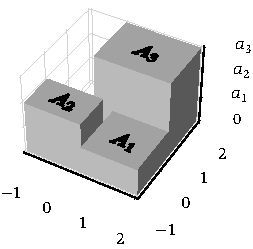
\includegraphics{figures/simple_function.pdf}
  \caption{\(\phi=a_1\indicator_{A_1}+a_2\indicator_{A_2}+a_3\indicator_{A_3}\)の模式図.}
\end{figure}

\begin{wrapfigure}[8]{o}{0pt}
  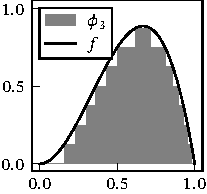
\includegraphics{figures/integration.pdf}
\end{wrapfigure}

より具体的に,\(\int f\measured{\mu}\)を非負値単関数の積分に関する極限で表すこともできる.\(\midx{E}{n}{k}=\inv{f}{\coival{2^{-n}k}{2^{-n}(k+1)}}\)とする.このとき
\[
  \phi_n = n\indicator_{\inv{f}{\ccival{n}{+\infty}}}+\sum_{k=0}^{2^nn-1}\frac{k}{2^n}\indicator_{\midx{E}{n}{k}}
\]
は非負値単関数で,\(\int\phi_n\measured{\mu}\to\int f\measured{\mu}\)(\(n\to\infty\))である.

\(f\)が負の値をとりうる可測関数のときは,\(f^{\mathord{+}}(x)=\max\Set{f(x),0}\)と\(f^{\mathord{-}}(x)=\max\Set{-f(x),0}\)が非負値可測関数であることを利用して
\[
  \int f\measured{\mu} = \int f^{\mathord{+}}\measured{\mu}-\int f^{\mathord{-}}\measured{\mu}
\]
と定義する.ただし,\(\int f^{\mathord{-}}\measured{\mu}=\int f^{\mathord{+}}\measured{\mu}=+\infty\)のとき\(\int f\measured{\mu}\)は定義されない.
\(\int f^{\mathord{-}}\measured{\mu}\)と\(\int f^{\mathord{+}}\measured{\mu}\)がどちらも有限なとき,\(f\)は\termdef{可積分}\index{かせきぶん@可積分}(integrable)であるという.

また,集合\(S\in\sigmaalg{F}\)上での積分は
\[
  \int_Sf\measured{\mu} = \int_Sf(x)\measured[x]{\mu}
  = \int f(x)\indicator_S(x)\measured[x]{\mu}
\]
で定義される.

特に\((\Omega,\sigmaalg{F},\prob)\)が確率空間のとき,確率変数\(X\)の積分\(\int X(\omega)\measured[\omega]{\prob}\)を\(X\)の\termdef{期待値}\index{きたいち@期待値}\index{EX@\(\expval[X]\)}(expected value)といい,\(\expval[X]\)と書く.

\begin{example}
  \cref{example:equally_possible}の確率空間\((\Omega,\sigmaalg{F},\prob)\)において,各\(\omega\in\Omega\)に対し\(X(\omega)\)を\(\omega\)の目で定義する.すなわち\(X(\dicei)=1\),\(X(\diceii)=2\)のようにする.
  このとき\(X=1\indicator_{\Set{\dicei}}+2\indicator_{\Set{\diceii}}+\dots+6\indicator_{\Set{\dicevi}}\)だから
  \[
    \expval[X] = 1\prob({\Set{\dicei}})+2\prob(\Set{\diceii})+\dots+6\prob({\Set{\dicevi}})
    = \frac{1+2+\dots+6}{6}
    = \frac{7}{2}
  \]
  である.この場合,\(\expval[X]=7/2\)は公平な6面ダイスの出目の期待値に相当する.
\end{example}

\begin{proposition}{}{}
  実数値関数\(f\)は有界閉区間\(I=\ccival{a}{b}\)上で定義され有界とする.このとき,\(f\)がリーマン積分できれば\(f\)はルベーグ可測かつ可積分で
  \[
    \int_a^bf(x)\intd{x} = \int_If\measured{\lambda}\quad\text{(\(\lambda\)は\(\numset{R}\)上のルベーグ測度)}
  \]
  が成立する.
\end{proposition}

\subsection{収束定理}

\begin{theorem}{単調収束定理}{monotone_convergence}\index{たんちょうしゅうそくていり@単調収束定理}\index{MCT|see{単調収束定理}}
  \((\Omega,\sigmaalg{F},\mu)\)を測度空間とする.可測関数列\(\seq{f_n}_{n\in\numset{N}}\)が\(0\leq f_1\leq f_2\leq\dotsb\)を満たすとき
  \[
    \lim_{n\to\infty}\int f_n(x)\measured[x]{\mu} = \int\pqty*{\lim_{n\to\infty}f_n(x)}\measured[x]{\mu}
  \]
  である.これを\termdef{単調収束定理}(monotone convergence theorem; MCT)という.
\end{theorem}

\begin{theorem}{ファトゥの補題}{fatou}\index{ふぁとうのほだい@ファトゥの補題}
  \((\Omega,\sigmaalg{F},\mu)\)を測度空間とする.任意の可測関数列\(\seq{f_n}_{n\in\numset{N}}\)に対して
  \[
    \int\pqty*{\liminf_{n\to\infty}f_n(x)}\measured[x]{\mu} \leq \liminf_{n\to\infty}\int f_n(x)\measured[x]{\mu}
  \]
  である.これを\termdef{ファトゥの補題}(Fatou's lemma)という.
\end{theorem}

\begin{theorem}{優収束定理}{dominated_convergence}\index{ゆうしゅうそくていり@優収束定理}\index{DCT|see{優収束定理}}
  \((\Omega,\sigmaalg{F},\mu)\)は測度空間で,可測関数列\(\seq{f_n}_{n\in\numset{N}}\)は関数\(f\)に各点収束するとする.
  このとき,可測関数\(g\)ですべての\(n\in\numset{N}\)に対し\(\abs{f_n}\leq g\)を満たすものが存在すれば
  \[
    \lim_{n\to\infty}\int f_n\measured{\mu} = \int f\measured{\mu}
  \]
  である.これを\termdef{優収束定理}(dominated convergence theorem; DCT)という.
\end{theorem}

\end{document}
